\documentclass[11pt,dvipdfmx]{jarticle}

\usepackage{eee}

\begin{document}
% トップページを書く
\begin{jikkenTitle} % この行で全体の枠を表示
 \gakunen{3} % 学年を記述。学年によって予定日部分の記載は異なる
 \numTitle{2}{実験レポートスタイルファイルの使い方} % 実験番号、タイトルを記述
 \subTitle{} % サブタイトルがあれば記述
 \jikkenbi{平成28年4月14日(木)} % 実験日を記述
 \jikkenbiII{平成28年4月21日(木)} % 実験日を記述(二日目がある場合。ない場合はこの行をコメントアウト)
 \kyoudou{電気電子工学コース教員} % 共同実験者名を記述
 \kyoudouII{その他の共同実験者} % その他の共同実験者名を記述

%%% 4年以外の場合(4年はコメント) %%%
 \yoteibi{4/28}% 予定日を記述
 \yoteibiII{5/12}% 予定日2を記述
 \yoteibiIII{5/19}% 予定日3を記述

%%% 4年の場合(4年以外はコメント) %%%
% \preYoteibi{4/28} % プレレポート予定日
% \preYoteibiII{5/12} % プレレポート予定日2
% \preYoteibiIII{5/19} % プレレポート予定日3
% \mainYoteibi{5/12} % メインレポート予定日
% \mainYoteibiII{5/19} % メインレポート2予定日
% \mainYoteibiIII{5/26} % メインレポート3予定日
 \hanNumberName{4}{3399}{小林 弘幸} % 班番号・学生番号・氏名を記述。この行でタイトルページの描画を終了
\end{jikkenTitle}

\section{目的}

電気電子工学コースのカリキュラム変更に伴い、2 年生の実験実習で \LaTeX のテーマを取り扱わなくなった。
このため、3 年生の情報処理IIの授業で \LaTeX の学習を行うことにする。
せっかく、実験実習のレポートがコンピュータで記述可能になるので、電気電子工学コースオフィシャルの実験実習レポートスタイルファイル(以下 eee.sty と呼ぶ)を配布することにした。
この文章の目的は、実験実習レポートスタイルファイルの使い方を述べると共に、簡単な \LaTeX の使い方を示す。
また、学生が陥りがちなハマリポイントなども記述する。

\section{スタイルファイルについて}

ここでは、eee.sty の中で記述したマクロの説明と、挿入したパッケージの使い方を説明する。
\subsection{表紙の記述方法}

eee.sty では、表紙を出力する環境を設定している。
\wpro{howToWriteTitle}は表紙を出力するためのソースコードである。
\verb+jikkenTitle+環境は表紙を書くための環境である。この環境内に\verb+\gakunen+から\verb+\hanNumberName+までのコマンドを記述することで表紙が記述できる。各コマンド引数はコメントで書いてあるので参考にすること。

\begin{lstlisting}[language={[LaTeX]TeX},caption=表紙記述方法,label=pro:howToWriteTitle]
\begin{jikkenTitle}
 \gakunen{3} % 学年を記述。この行で全体の枠を表示
 \numTitle{2}{実験レポートスタイルファイルの使い方} % 実験番号、タイトルを記述
 \subTitle{} % サブタイトルがあれば記述
 \jikkenbi{平成28年4月14日(木)} % 実験日を記述
 \kyoudou{電気電子工学コース教員} % 共同実験者名を記述
 \yoteibi{4/21}% 予定日を記述
 \hanNumberName{4}{3399}{小林 弘幸} % 班番号・学生番号・氏名を記述。この行でタイトルページの描画を終了
\end{jikkenTitle}
\end{lstlisting}

\subsection{参照の方法}
\label{sec:reference}

\LaTeX では節・図・表・式には\verb+\label+コマンドでラベルを付けて、\verb+\ref+コマンドで参照する。ラベル名はユニークである必要があるので、同じラベル名を図と表に付けることはできない。そこで、eee.sty では以下のようにラベルを付けることを推奨する。
\begin{description}
 \item [節の場合] \verb+\label{sec:節ラベル}+
 \item [図の場合] \verb+\label{fig:図ラベル}+
 \item [表の場合] \verb+\label{tab:表ラベル}+
 \item [式の場合] \verb+\label{eq:式ラベル}+
 \item [プログラムの場合] \verb+\label{pro:プログラムラベル}+
\end{description}

\wptab{reference}は、このようにラベルを付けたときの参照用のマクロとその結果である。これらのコマンドによって、図・表などの接頭子を付ける必要がなくなるだけでなく、式の()を付け忘れずにすむ。「X」の部分には「fig:」や「tab:」などの接頭子を除いたものを記述する。
\begin{table}[tbp]
 {\small
  \centering
  \caption{eee.sty の参照系マクロとその結果}
  \label{tab:reference}
  \begin{tabular}{|c|c||c|c|c|c|c|}\hline
   \multirow{2}{*}{通常}
   & マクロ
   & \verb+\wfig{X}+
   & \verb+\wtab{X}+
   & \verb+\weq{X}+
   & \verb+\wsec{X}+
   & \verb+\wpro{X}+
   \\ \cline{2-7}
   & 結果
   & 図x
   & 表x
   & 式(x)
   & \bf{x}
   & プログラムx
   \\ \hline
   \multirow{2}{*}{ページ付}
   & マクロ
   & \verb+\wpfig{X}+
   & \verb+\wptab{X}+
   & \verb+\wpeq{X}+
   & \verb+\wpsec{X}+
   & \verb+\wppro{X}+
   \\ \cline{2-7}
   & 結果
   & pページ図x
   & pページ表x
   & pページ式(x)
   & pページ\bf{x}
   & pページプログラムx
   \\ \hline
  \end{tabular}
 }
\end{table}


\subsection{プログラムリストの記述方法}

eee.sty では jlisting パッケージを入れている。プログラムリストを出力する方法は以下の二つである。
\begin{itemize}
 \item \verb+\lstlisting+ コマンドで外部に記述されたソースコードを直接取り込む
 \item \verb+lstlisting+ 環境内にプログラソースを記述する
\end{itemize}

\wpro{howToIncludeProgram}は、外部のソースコードを取り込む記述法である。
実験などでは個別にプログラムをファイルで保存していると思うので、いちいち文書内に同じことを書かなくてよいのでこの手法が一番便利だと思う。
なお、このようにして取り込んだ結果を\wpro{helloWorld}に示す。
言語を C に設定したので、コメントが斜体になっていたり、予約後が太字になっていたりしている。
\begin{lstlisting}[language={[LaTeX]TeX},caption=外部のソースコードを取り込む方法,label=pro:howToIncludeProgram]
% [] 内にオプションを付けられる
% langage は表示したい言語
% caption はタイトル
% label はラベル。コンフリクトしないように pro: を付けておく
% {} の中に記述したいファイル名を書く
\lstinputlisting[language=C,caption=Hello World.c,label=pro:helloWorld]{hello.c}
\end{lstlisting}

\lstinputlisting[language=C,caption=Hello World.c,label=pro:helloWorld]{hello.c}

一方、自分で作成したわけではなく、原理などでちょっとしたプログラムを書きたい場合には、\wpro{howToInlineProgram}のように\verb+lstlisting+環境内に直接プログラムを記述する。外にプログラムのソースファイルを用意する必要がないので、説明だけのコードの場合にはこちらの方が便利だと思う。

なお、このようにして取り込んだ結果を\wpro{initMethod}に示す。
ここでは、Ruby 言語を選択しているので、def や end などの予約後が太字になっていることが確認できる。

\lstinputlisting[language={[LaTeX]TeX},caption=直接プログラムを記述する方法,label=pro:howToInlineProgram]{inlineRuby.tex}

\input{inlineRuby.tex}

\subsection{グラフの描画}
\wtab{ohmData}のデータをサンプルとして、グラフの描画方法を示す。
グラフを描画するソフトウェアは沢山あるが、ここでは情報処理Iで使用したフリーソフトの gnuplot で描画する例を示す。

\begin{table}
 \centering
 \caption{ある回路における電圧・電流の関係}
 \label{tab:ohmData}
 \begin{tabular}{|c||c|c|c|c|c|c|c|c|c|}\hline
  電圧$v[V]$ & 0.0 & 10.0 & 20.0 & 30.0 & 40.0 & 50.0 & 60.0 & 70.0 & 80.0 \\ \hline
  電流$i[A]$ & 0.00 & 0.99 & 2.02 & 3.07 & 3.95 & 4.93 & 6.01 & 7.10 & 7.98 \\ \hline
 \end{tabular}
\end{table}

まず、\wtab{ohmData}の電圧・電流値を\wpro{jikken.txt}に示すように\verb+jikken.txt+というファイルに保存する。グラフを書く度にコマンドを入力するのは面倒なので、\wpro{graph1.gp}に示すコマンド記述ファイル(\verb+graph1.gp+)を作成する。

\lstinputlisting[language=C,caption=実験データテキスト,label=pro:jikken.txt]{jikken.txt}
\lstinputlisting[language=C,caption=Gnuplotコマンドファイル(1),label=pro:graph1.gp]{graph1.gp}

ここまで準備できたら、コマンドラインから\verb+gnuplot graph1.gp+とすることで、\wfig{graph1}に示す graph1.pdf ファイルを作成することができる。
ここで作成された PDF ファイルは\verb+\includegraphics+コマンドを使って\LaTeX に取り込むことができる。
ただし、LaTeX のプログラムは PDF ファイルのサイズを知ることができないので、あらかじめ次のコマンドで\verb+graph1.xbb+ファイルを作成しておく(xbb ファイルについては、環境によっては簡単に作成できたり、作成しなくてもよい場合があるので、詳細を付録で説明する)。
\begin{verbatim}
extractbb graph1.pdf
\end{verbatim}

\input{inputGraph1}

ここまで周辺ファイルが準備できたら、\LaTeX ソースファイル内に\wpro{howToIncludeGraph}のように記述する。
このようにして記述した結果が\wfig{graph1}である。
figure 環境の中に\verb+\begin{center}〜\end{center}+を入れると上下に余計な空白が入ってしまうので、\verb+\centering+を使うようにする(ネットの説明などでは center 環境が紹介されていることが多いので鵜呑みにしないこと)。
また、includegraphics のオプションを付けることで、図の大きさを設定することができる。
ここでは、幅として width を設定しているので、高さは挿入される画像の比率から自動的に設定される。
width 以外にも scale など様々なオプションがあるので、自分で調査すること。

\lstinputlisting[language={[LaTeX]TeX},caption=PDF ファイルを埋め込む方法,label=pro:howToIncludeGraph]{inputGraph1.tex}

\wfig{graph1}は情報処理Iの授業で習ったように点同士を直線で結んでいる。
このためグラフがポイントの部分で折れ曲がっていることがわかる。
この例はオームの法則の実験データを示していると思われるため、できれば実験で習ったように直線で近似したい。

このような場合に対応するように gnuplot では近似直線や近似曲線を描くことができる。
\wpro{graph2.gp}は近似直線のパラメータを推定する gnuplot スクリプトを示している。
このスクリプトでは、実際のデータをポイントで描画し、近似直線を実線で同時に描画している。このスクリプトで作成された図を\wfig{graph2}に示す。

\lstinputlisting[language=C,caption=Gnuplotコマンドファイル(2),label=pro:graph2.gp]{graph2.gp}

\begin{figure}[tbp]% 図の環境を開始(top, bottom, pageの順で配置を試みる)
 \centering% 環境をセンタリング
 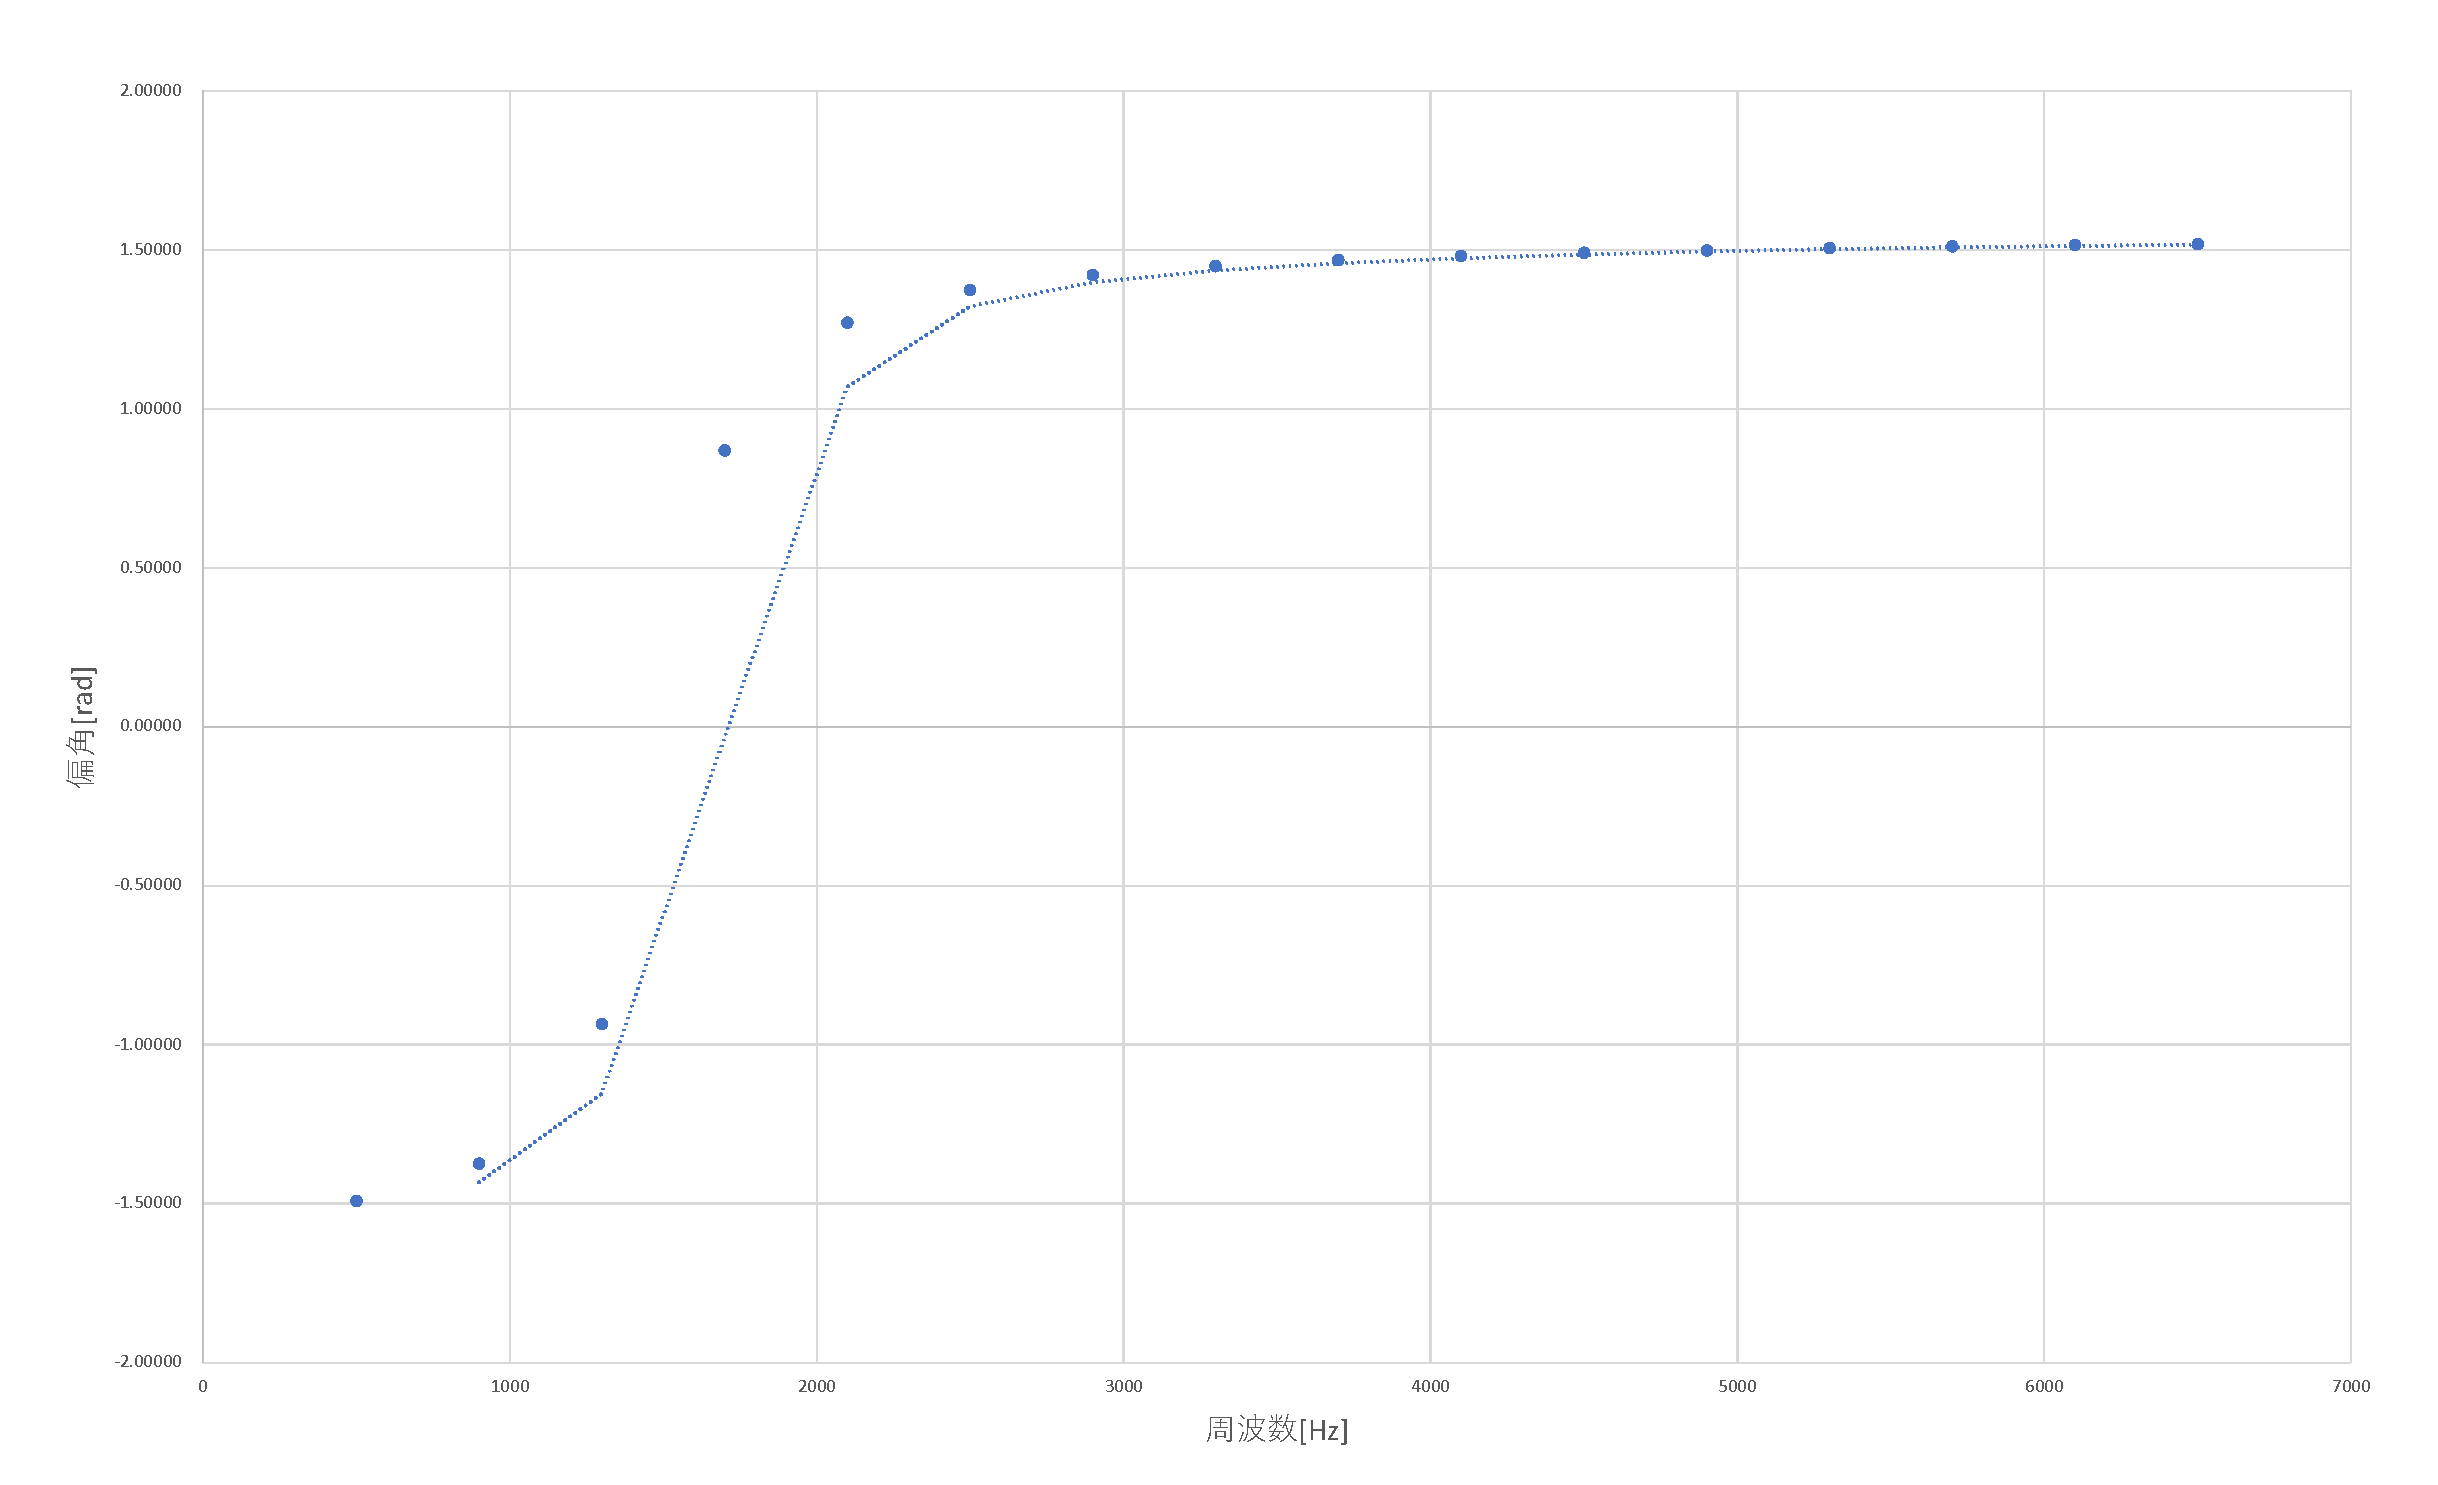
\includegraphics[width=10cm]{graph2.pdf}% pdf を挿入
 \caption{近似直線の描画}% キャプションを記述
 \label{fig:graph2}% 図のラベルを設定
\end{figure}% 図の環境を終了

\newpage
\wpro{sample.gp}は gnuplot のサンプルファイルを出力するための gnuplot スクリプトである。
ここでは、せっかくなので、サンプル出力を A4 用紙全体に寝かせた形で出力してみる(landscape モード)。
実験によっては、グラフをA4横で出力するように指示がされる場合があるので、参考にして欲しい(個人的には反対方向に90度回転の方が好みなのだが、lscape スタイルファイルにおいてハードコーディングされているので仕方ない)。

\lstinputlisting[language=C,caption=Gnuplotサンプル出力方法,label=pro:sample.gp]{sample.gp}
\lstinputlisting[language={[LaTeX]TeX},caption=90度回転したグラフ出力,label=pro:sample]{importLandscape.tex}

\input{importLandscape}

\subsection{数式の書き方}
文中の数式は\verb+$+と\verb+$+で括ればよい。\verb+$x$+と書くと$x$のようになる。一方、数式だけの行を書くのであれば、\verb+\begin{equation}+と\verb+\end{equation}+で括る。この場合、式番も自動的に付き、\verb+\weq{}+コマンドで「\weq{2次方程式}」のように参照できる。
\begin{equation}
 y = f(x) = x^2 + 2x + 1 \label{eq:2次方程式}
\end{equation}

複数行の数式を書く場合には align 環境を使う。この時、\verb+\\+ で改行を行い、\verb+&+ マークで各行の横位置を揃えることができる。align の場合、式番はすべての行に自動的に振られてしまう。例えば、下の例のように式が等号で連続して繋がる場合には、\verb+\nonumber+を使い式番を付けないようにする。実際の書き方は、このプログラムのソースを見ること。ただし、align を使うには amsmath を usepackage する必要がある(このスタイルファイルを使えば自動的に入る)。
\begin{align}
   y &= \int\left(\int-g dt\right) dt \nonumber \\
   &= \int(-gt + C_1)dt \nonumber \\
   &= -\frac{1}{2}gt^2 + C_1t + C_2
\end{align}

\appendix
\section{付録}

\subsection{外部ファイル読み込みの例}
非常に長いプログラムを挿入した場合の例として、\wpro{eee.sty}に eee.sty を読み込んだ結果を示す。
\lstinputlisting[language={[LaTeX]TeX},caption=eee.styの中身,label=pro:eee.sty]{eee.sty}

\end{document}

